%==============================================================================
%  CS 613 NLP --- Assignment 2 --- Merged Final Report
%  Compile with:  tectonic final_draft.tex   (or Overleaf / pdflatex + bibtex)
%==============================================================================
\documentclass[10pt,a4paper]{article}

%------------------------------ Fonts & type ----------------------------------
\usepackage[T1]{fontenc}
\usepackage[utf8]{inputenc}
\usepackage{amsmath,amssymb,mathtools}  % must precede newtxmath
\usepackage{newtxtext,newtxmath}   % compact Times-like text + matching math
\usepackage{microtype}             % protrusion/expansion -> better justification
\usepackage{setspace}
\setstretch{1.11}
\setlength{\parskip}{2.5pt plus .5pt minus .5pt}
\setlength{\parindent}{1.4em}
\renewcommand{\arraystretch}{1.06}

%------------------------------ Page geometry --------------------------------
\usepackage[a4paper,left=2.4cm,right=2.4cm,top=2.2cm,bottom=2.3cm,
            headheight=19pt]{geometry}

%------------------------------ Tables & figures -----------------------------
\usepackage{booktabs}
\usepackage{array}
\usepackage{tabularx}
\newcolumntype{L}[1]{>{\raggedright\arraybackslash}p{#1}}
\usepackage{makecell}
\usepackage{multirow}
\usepackage{graphicx}

%------------------------------ Colour & links -------------------------------
\usepackage{xcolor}
\definecolor{linkblue}{HTML}{1F4E79}
\definecolor{citegreen}{HTML}{2E6B3E}
\definecolor{rulecol}{HTML}{9AA5B1}

%------------------------------ Lists ----------------------------------------
\usepackage{enumitem}
\setlist{nosep,leftmargin=1.5em,topsep=2pt,itemsep=1.5pt}

%------------------------------ Headings -------------------------------------
\usepackage{titlesec}
\titleformat{\section}{\large\bfseries\color{linkblue}}{\thesection}{0.6em}{}
\titleformat{\subsection}{\normalsize\bfseries}{\thesubsection}{0.55em}{}
\titleformat{\subsubsection}{\small\bfseries}{\thesubsubsection}{0.5em}{}
\titleformat{\paragraph}[runin]{\bfseries}{}{0em}{}[.]
\titlespacing*{\section}{0pt}{1.9ex plus .3ex}{0.85ex}
\titlespacing*{\subsection}{0pt}{1.4ex plus .2ex}{0.5ex}
\titlespacing*{\paragraph}{0pt}{0.8ex plus .2ex}{0.55em}

%------------------------------ Captions -------------------------------------
\usepackage{caption}
\captionsetup{font=small,labelfont=bf,skip=6pt,width=0.98\textwidth}

%------------------------------ Header / footer ------------------------------
\usepackage{fancyhdr}
\pagestyle{fancy}
\fancyhf{}
\fancyhead[L]{\footnotesize\itshape CS\,613 NLP --- Assignment\,2}
\fancyhead[R]{\footnotesize\itshape Adjacent-Layer Merging of GPT-2}
\fancyfoot[C]{\footnotesize\thepage}
\renewcommand{\headrulewidth}{0.3pt}
\renewcommand{\headrule}{\hbox to\headwidth{\color{rulecol}\leaders\hrule height \headrulewidth\hfill}}

%------------------------------ Hyperlinks (load last) -----------------------
\usepackage[colorlinks=true,linkcolor=linkblue,citecolor=citegreen,
            urlcolor=linkblue]{hyperref}
\hypersetup{
  pdftitle={Depth Compression of GPT-2 Small by Adjacent-Layer Merging},
  pdfauthor={Sumit Kumar Jha, Amrita Lodh, Hiroyoshi Tsujimoto,
    Sura Sravan Kumar, Satvik Sharma, Lingala Hasini}
}

%------------------------------ Tighten display math -------------------------
\AtBeginDocument{%
  \setlength{\emergencystretch}{2.2em}%
  \setlength{\abovedisplayskip}{4pt plus 2pt minus 2pt}%
  \setlength{\belowdisplayskip}{4pt plus 2pt minus 2pt}%
  \setlength{\abovedisplayshortskip}{2pt}%
  \setlength{\belowdisplayshortskip}{2pt}%
}

%------------------------------ Bib ------------------------------------------
\usepackage{natbib}

%------------------------------ Macros ---------------------------------------
\newcommand{\dropfirst}{\textsc{drop-first}}
\newcommand{\dropsecond}{\textsc{drop-second}}
\newcommand{\ce}{\mathrm{CE}}
\newcommand{\removeop}{\texttt{Remove}}
\newcommand{\averageop}{\texttt{Average}}
\newcommand{\linop}{\texttt{LinearMultiply}}
\newcommand{\nlop}{\texttt{NonlinearMultiply}}
\newcommand{\slerp}{\mathrm{slerp}}
\newcommand{\term}{\textsc{TerGRASP}}

\begin{document}

%==============================================================================
% Title block
%==============================================================================
\begin{center}
{\LARGE\bfseries Depth Compression of GPT-2 Small by Adjacent-Layer Merging\par}
\vspace{0.35em}
{\large A Unified Comparison of Learnable Weight-Space Merging, Iterative
Operator Search, Affine Composition, and Similarity-Guided SLERP\par}
\vspace{0.9em}
{\normalsize
\begin{tabular}{@{}c@{\hspace{2.4em}}c@{\hspace{2.4em}}c@{}}
Sumit Kumar Jha & Amrita Lodh & Hiroyoshi Tsujimoto\\[0.15em]
{\normalsize\ttfamily sumitjha@iitgn.ac.in} &
{\normalsize\ttfamily amrita@iitgn.ac.in} &
{\normalsize\ttfamily hiroyoshi@iitgn.ac.in}\\[1.1em]
Sura Sravan Kumar & Satvik Sharma & Lingala Hasini\\[0.15em]
{\normalsize\ttfamily sravan@iitgn.ac.in} &
{\normalsize\ttfamily satvik@iitgn.ac.in} &
{\normalsize\ttfamily lingala@iitgn.ac.in}
\end{tabular}\par}
\vspace{0.9em}
{\small CS\,613: Natural Language Processing \quad$\cdot$\quad Indian Institute
of Technology Gandhinagar\par}
\vspace{0.3em}
{\footnotesize\itshape Code: \url{https://github.com/sumitjhaa/gpt2-layermerging/tree/main/Assignment2}\par}
\end{center}

\vspace{-0.4em}
\hrule height 0.4pt
\vspace{0.6em}

%==============================================================================
\begin{abstract}
\small
We compressed GPT-2 Small ($124{,}439{,}808$ parameters across twelve
transformer blocks) by folding adjacent blocks into single ones, and we judged
the result by how much next-token perplexity we lost for each parameter saved.
After the first presentation the mentor told us to try many different merging
ideas, because adjacent-layer merging is barely explored; one rule held
everywhere---only adjacent layers may be merged. Six of us covered the space:
four main experiments, one tangential study that mapped the field and produced
the baselines everyone else used, and a short pilot. Every experiment ran on
the same WikiText-2 split for training and selection and the same three one-shot
tests, DBpedia-14, AG News and IMDb, opened only at the very end.

Put simply, trained merges win. A learnable weight-space merger
(Experiment~A) beats plain deletion at every compression level and degrades
gracefully instead of collapsing; a trainable block (Experiment~B) is the best
method in $14$ of $15$ unseen stage$\times$dataset cells. Averaging does not
work, because the neurons of two adjacent blocks are not aligned, and the cost
at five merges runs from $+1{,}385\%$ (Experiment~B) to $+83{,}745\%$
(Experiment~A) in perplexity. Training-free rules are messier: affine
composition with calibration-based selection (Experiment~C) and calibrated
SLERP (Experiment~D) both beat deletion at one or two merges, but the winner
changes with the pair and the model. Every per-pair ranking and control is in
the body; the experiment we would run next is the same merging on a
multilingual backbone.
\end{abstract}

\hrule height 0.4pt
\vspace{0.4em}

%==============================================================================
\section{Introduction}
%==============================================================================

Decoder-only Transformer language models
\citep{vaswani2017attention,radford2019language} store a large fraction of
their parameters in \emph{depth}. For GPT-2 Small each transformer block holds
$5{,}898{,}240$ parameters ($4\times768^2$ attention projections,
$2\times768\times3072$ MLP projections, biases and two LayerNorm vectors), so
removing $k$ of the $12$ blocks removes $5.90k$M of $124.44$M parameters. Depth
compression is attractive because it reduces both memory and sequential
latency, but naive removal of a block destroys the function that block computed.

We did this assignment as one team. After Presentation~1 the mentor told us
that adjacent-layer merging is a brand-new area and that the group should
tackle a \emph{wide variety} of experiments, with each member pursuing one
distinct idea; every method had to improve the perplexity--parameter-reduction
trade-off, and non-adjacent layers must never be merged. Rather than have all
six of us chase the same method, we agreed on a division of labour: each
member designed and ran one distinct merging family under a shared protocol,
and everyone's numbers are reported together here. The sections that follow
are that merged write-up. Experiment~A (Amrita) is a learnable
\emph{weight-space hypernetwork} that reads two adjacent blocks and emits dense
additive corrections to the retained block, under a guarded deployment rule.
Experiment~B (Hiroyoshi) is an \emph{iterative}, stage-wise operator search
that compares deletion, averaging, closed-form affine composition and a
trainable block under one exact evaluator. Experiment~C (Lingala) is
\emph{affine} merging with a similarity-gated, error-weighted SLERP operator
(SG-SC) and a calibration-guided operator selector (CGOS). Experiment~D
(Sravan) is a \emph{calibrated}, similarity-guided SLERP merger whose
per-module merge weights are tuned on a small calibration split. Sumit's
foundational exploration is a tangential sweep of fifteen approaches that
established the reference baselines---Block-Influence removal, pruned
distillation, LayerDrop, a fitted ternary bridge---and the negative results
that define the problem. Satvik's pilot covers the closed-form training-free
merges (Union-Select-Reconstruct, Remove-and-Patch, Correlation-Guided Neuron
Fusion).

\paragraph{Contributions.}
We ran everything under one protocol---WikiText-2 for training and selection,
with DBpedia-14, AG News and IMDb opened exactly once---so the four families
can be compared on equal terms. The headline results, in order: a learned
merger that beats deletion by up to $1.82$ nats of validation cross-entropy at
equal compression and reaches $68.23$ IMDb perplexity at $28.48\%$ removal
(Experiment~A); a controlled five-stage comparison in which a trainable block
is best in $14$ of $15$ unseen stage$\times$dataset cells (Experiment~B); two
training-free methods that beat deletion at low compression, affine
composition with CGOS at $47.93$ test perplexity (Experiment~C) and a
calibrated SLERP at $43.85$ (Experiment~D); and, at the level of how things go
wrong, an explanation for why averaging fails (neuron permutation) and why
local affine fitting does not automatically help---removability and residual
low-rankness are different properties.

%==============================================================================
\section{Report}
%==============================================================================

\subsection{Mentor Feedback Since Presentation 1}
\label{sec:feedback}

The study is organised around the feedback received after Presentation~1 and in
the weekly mentor meetings.

\begin{itemize}
  \item \emph{Presentation~1 follow-up (group-wide).} The mentor asked us to
    ``tackle a wide variety of experiments'' because he sees adjacent-layer
    merging as a brand-new branch of research, subject to the hard constraint that
    \emph{only adjacent layers may be merged}, and that the group must improve
    both perplexity and the parameter-reduction rate. We spread the work so
    that each member owns one distinct operator family (weight-space
    hypernetwork, iterative operator comparison, affine/CGOS, calibrated SLERP,
    and training-free closed-form merges) and the portfolio covers the design
    space.
  \item \emph{Follow-up (multilingual).} The mentor noted that applying
    adjacent merges to \emph{multilingual} models is interesting. That is why
    every operator here is backbone-agnostic, and why we name multilingual
    transfer as the primary follow-up (Section~\ref{sec:limits}).
  \item \emph{Week~1.} A learned merger must not be compared against a
    straw-man, and reconstruction loss alone is not evidence of
    language-modelling quality. We therefore let Experiment~A start from
    \dropfirst{} exactly---its learned correction is zero-initialised---and
    added a temperature-scaled KL term; Experiment~B promotes \removeop{} to a
    first-class operator under one exact evaluator.
  \item \emph{Week~2.} An approximate scorer could bias the comparison.
    Every experiment moved to exact, token-weighted sliding-window perplexity,
    and Experiment~B added SHA-256 hashes to lock the protocol.
  \item \emph{Week~3.} Demonstrate that merge semantics are correct before
    trusting results, and isolate selection from test. Experiment~A gained a
    preflight equality check and a disjoint ranking partition; Experiment~B
    runs five structural self-checks on a tiny GPT-2; Experiments~C and~D carve
    calibration/window holdouts and touch the test set once.
  \item \emph{Week~4.} Hyperparameter ablation and explicit computational
    resources. Each experiment carries a targeted ablation (Tables
    \ref{tab:batch}\,\&\,\ref{tab:gap} for~A; \ref{tab:ablation-b} for~B;
    SG-SC/rank sweeps for~C; a weight-mode grid for~D) and a resources
    paragraph (Section~\ref{sec:management}).
  \item \emph{Week~5.} Keep the evaluation protocol identical across methods
    and state limitations honestly. We converged on one shared evaluator and
    committed to saying plainly where the evidence is thin;
    Section~\ref{sec:limits} does that.
\end{itemize}

\subsection{Baselines and State of the Art}
\label{sec:sota}

Depth reduction in Transformers has moved from simply deleting layers to
learning how to fuse them, and we grouped the relevant work into four families,
treating the closest members as explicit baselines.

\paragraph{Layer removal.} \citet{gromov2024unreasonable} show that the deeper
layers of decoder-only Transformers are often redundant and can be deleted with
little perplexity loss. \citet{men2024shortgpt} formalise this with the
\emph{Block Influence} (BI) score, the cosine similarity between a block's input
and output, and remove the least influential blocks. The \dropfirst{} control in
Experiments~A and~B, the \removeop{} operator in Experiments~B and~C, and the
foundational BI baseline are exactly this family.

\paragraph{Static layer merging.} \citet{yang2024laco} collapse rear layers into
preceding ones with the Reserving-Differences-while-Seeking-Common (RDSC) rule
and no training. \citet{liu2024pruning} identify mergeable layers by manifold
alignment in activation space and combine them by closed-form averaging. Both
use \emph{fixed} coefficients from a similarity heuristic. The \averageop{}
operator (Experiments~B, C, D) and the Random-Weight-Average control
(Experiment~C) represent this family.

\paragraph{Affine composition.} \linop{} (Experiment~B) fits a linear map from a
group's input to its output and absorbs the span into a single affine block,
composed layer-wise through Cholesky factors. It is the strongest
\emph{training-free} operator in the study and is related in spirit to the
closed-form composition used by \citet{yang2024laco}.

\paragraph{Learned fusion.} \citet{pei2024fusegpt} introduce FuseGPT, which
reframes pruning as knowledge redistribution: a redundant block is fused into a
neighbour using low-rank learnable matrices under a Macro Influence criterion
with lightweight local distillation. This is the closest SOTA and the
upper-reference target. Our learnable methods follow the same philosophy---the
merged artifact is \emph{trained} to reproduce the hidden states of the original
span plus a logit-level KL term \citep{hinton2015distilling}---but differ in
form: Experiment~A uses a weight-space hypernetwork with \emph{dense}
corrections, and Experiment~B uses a full trainable GPT-2 block.

\paragraph{Distillation and structured pruning.} \citet{sanh2019distilbert}
halve BERT's depth by distillation with every-other-layer initialisation.
Orthogonal structured methods delete rows/columns (SliceGPT,
\citealt{ashkboos2024slicegpt}) or non-critical channels (LLM-Pruner,
\citealt{ma2023llmpruner}); they do not reduce depth and serve as context,
although our distillation repairs follow the LLM-Pruner recipe.
\citet{fan2020layerdrop} fine-tune with structured layer dropout; we ran it as a
full competing method in the foundational exploration because it is the one
depth-reduction scheme with a public recipe. \citet{stoica2024zipit} merge
features within and across models, the closest relative of our fusion pilot.
The similarity-guided pair selection and adaptive merge weights of Experiments
C and~D are motivated by \citet{zhang2025com} and \citet{liu2024mka}, and the
ternary factor grid by \citet{ma2024bitnet}.

\paragraph{Availability of baseline implementations.} The removal and averaging
controls are implemented by us in full, so they need no external release. The
same is true of \linop{}, the four operators of Experiment~B, the SG-SC and CGOS
selectors of Experiment~C, the calibrated SLERP of Experiment~D, and the fifteen
foundational approaches; everything is directly comparable by construction. The
closest external method, FuseGPT, has no official public release, and its
low-rank fusion is tied to its own pruning schedule. We therefore position
against its \emph{idea} rather than a re-run, instantiating every reproducible
mechanism as a like-for-like control.

\subsection{Datasets}
\label{sec:datasets}

\paragraph{Training and selection data.} All learning, calibration and model
selection use only \textbf{WikiText-2} \citep{merity2016pointer}, loaded as
\texttt{Salesforce/wikitext}, config \texttt{wikitext-2-raw-v1}. Raw rows are
reassembled into whole articles where needed, exact duplicate articles are
removed, and the unique text is partitioned \emph{before} tokenisation into
disjoint train/checkpoint/ranking (A) or train/calibration/evaluation (C, D)
roles with a fixed permutation and seed; every partition and its hash are
recorded.

\paragraph{In-domain final evaluation.} The full official WikiText-2 validation
split is used only at the end and only for the selected configuration; the
scored-token counts range from $244{,}824$ (A) to $249{,}748$ (B) across
experiments because of small differences in boundary-token treatment. The
original model reaches $\mathrm{PPL}=29.37$ (A), $28.61$ (B), and $33.94$ (D, on
its own validation windows); we never compare absolute values across experiments
because the exact evaluators differ in window size and stride.

\paragraph{Out-of-domain test data.} We evaluate on three external test sets
chosen so that their relationship to WikiText-2 varies along two axes,
\emph{context} and \emph{tokens}, exactly as the assignment directs:
\emph{DBpedia-14} \citep{zhang2015character,lehmann2015dbpedia} (similar
context, different tokens), \emph{AG News} \citep{zhang2015character} (different
context, nearer tokens), and \emph{IMDb} \citep{maas2011learning} (different in
both). Each source is capped at a fixed token budget with a fixed seed
($32{,}768$ tokens in A; $400{,}000$ in B); labels are ignored and only
next-token prediction is scored. Because the corpora differ in content and token
cap, absolute perplexities are \emph{not} comparable across domains; we report
relative change over each corpus's own original GPT-2 baseline.

\paragraph{Bias handling.} WikiText-2 is a single-domain English Wikipedia
corpus, so selection can quietly inherit its lexical and topical biases. We
tried to keep that from contaminating the comparison. Articles are partitioned
before tokenisation at article granularity, so near-duplicates cannot leak
across roles, and exact duplicates are removed before the split. Model
selection never touches the official validation split or the external
corpora---A ranks on a disjoint holdout under a guarded acceptance rule, B
selects on validation and locks the test text with hashes, and C and D select
on calibration or holdout windows. Finally, unseen domains are reported
relative to their own GPT-2 baseline, so a vocabulary mismatch between corpora
cannot dress itself up as a compression effect.

\paragraph{Bottleneck.} The dominant bottleneck varies by experiment. In~A it is
GPU memory during logit materialisation, handled by scoring in chunks of $128$
tokens under activation checkpointing; the secondary bottleneck is the
exhaustive non-overlapping-set search for $k$ merges. In~B it is evaluation and
distillation cost, so each unseen corpus is capped and the evaluator batched; the
second bottleneck is \emph{stage-wise coupling}. In~C and~D it is the
calibration/activation pass and the affine solve. The foundational exploration's
bottleneck is that all fifteen approaches ran on one free Apple-Silicon MPS
laptop with no paid GPU, forcing $60$--$80$-step training budgets. The common
bottleneck is two shared six-hour-class accelerators, which caps training
passes.

\paragraph{Dataset extension and difference from the previous version.}
Relative to Presentation~1, which used a single WikiText-2 split, the data
pipeline changed in three ways. Articles are now re-partitioned into disjoint
roles with a fixed seed and hashes, so the selection holdouts cannot overlap
the training text. Three external corpora (DBpedia-14, AG News, IMDb) were
added as a one-shot unseen test along the two axes the assignment points at.
And small calibration budgets (${\sim}4$k--$20$k tokens) are carved out of the
\emph{train} split, so no fitted operator ever sees validation or test text.
The old setup could only measure in-domain fit; the new one measures held-out
selection and out-of-domain transfer separately. No new data were collected;
all corpora are public.

\subsection{Experimental Plan}
\label{sec:plan}

\paragraph{Research questions.}
We went in with four questions. First, whether a \emph{learned} artifact could
fold one block into its neighbour and still beat plain deletion on held-out
text. Second, which adjacent pairs are actually safe to merge, and whether the
ranking a model learns at home still holds once we move to out-of-domain data.
Third, how quality falls off as we keep merging, and whether the ordering
between operators survives into the unseen domains. Fourth, how close a
training-free rule can get to the learned methods, and whether a cheap
calibration signal agrees with validation-based selection.

\paragraph{Setting and robustness under limited compute.} Everything ran on shared
six-hour Kaggle/Colab sessions with two NVIDIA Tesla T4 GPUs ($15$\,GiB each),
$4$ vCPU cores, ${\sim}13$\,GiB RAM and ${\sim}20$\,GiB scratch, plus the
Apple-Silicon laptop for the foundational grid. Within that budget we stayed
robust by mixing training tasks so that every pair and compression level
appears in a single pass (A), by capping the external corpora and batching the
evaluator rather than shortening training (B), by preferring closed-form fits
wherever one exists (B, C, D and the pilot), and by deriving every stochastic
fit from an explicit per-fit generator whose seeds are recorded
(foundation).

\paragraph{How the approaches differ.} The four primary experiments are
separated by \emph{mechanism}, not by incidental implementation. What gets
learned or selected changes across them: a dense additive correction in
\emph{weight space} (A), a full replacement block in \emph{activation space}
(B), a closed-form affine map \emph{picked} by calibration (C), or a per-module
\emph{interpolation weight} on a spherical path (D). The search differs too,
from exhaustive non-overlapping-set selection (A) and a greedy stage-wise
boundary search (B) to per-pair then joint selection (C) and greedy
similarity-guided iteration (D). So does the compute: gradient training of a
hypernetwork and of a single block in A and B, versus the training-free
closed-form and interpolation operators of C, D and the pilot. The dependent
variable stays the same everywhere---next-token cross-entropy, reported as
perplexity, with top-1/top-5 accuracy and parameter count as secondary
measures.

\paragraph{Model architectures and parameter counts.} All experiments operate on
GPT-2 Small: $n_\text{layer}=12$, $d=768$, $12$ heads, vocabulary $50{,}257$,
tied input/output embedding, learned positional embeddings, and \texttt{Conv1D}
projections stored as $[\text{in},\text{out}]$; the total is $124{,}439{,}808$
parameters and each block holds $5{,}898{,}240$. Merged artifacts differ in
size: A's training-time hypernetwork holds $39{,}391{,}168$ parameters (discarded
at deployment); B's \nlop{} holds one block's parameters; C's affine map holds
$768^2+768$ parameters while dropping the rest of the block; D's SLERP added no
new parameters in the reported runs; the pilot's low-rank patch holds
${\sim}2dr$ parameters; and the foundational ternary bridge holds ${\sim}2dr$
weights at ${\sim}1.58$ bit/param. Deployed compressed models after $k$ merges
hold $124{,}439{,}808-5{,}898{,}240\,k$ parameters (viz.\ $117{,}351{,}936$ at
$k=1$ and $89{,}000{,}448$ at $k=5$).

\paragraph{Hyperparameter search and ablation.} A full grid is infeasible on the
shared GPUs, so we run targeted ablations and state explicitly what is fixed:
\emph{(A)} an exact throughput-and-memory sweep over global batch size
(Table~\ref{tab:batch}) and a training-length sweep reading the equal-level CE
gap per epoch (Table~\ref{tab:gap}), all other weights fixed
(Table~\ref{tab:ablation}); \emph{(B)} a targeted ablation on the nonlinear
training length (Table~\ref{tab:ablation-b}); \emph{(C)} SG-SC component
ablations, a rank/direction sweep, and CGOS vs.\ validation selection;
\emph{(D)} a merge-weight/mode grid (fixed-$0.5$ linear, similarity-prior SLERP,
calibrated shared weight, calibrated per-group weights with mode search); and
the \emph{foundation} a rank/bitwidth sweep with a random-removal control.

\paragraph{Metric choice and justification.} The primary metric is mean
next-token cross-entropy and its exponential, perplexity. Cross-entropy is the
right scalar because the task is pure language modelling: it is additive over
positions and strictly proper, so a model cannot be rewarded for a confidently
wrong distribution. Perplexity is reported alongside as the conventional unit in
depth-pruning work and is used only for \emph{within-corpus} comparisons.
Beyond that we also kept an eye on top-1 and top-5 next-token accuracy over the
same sliding windows, the paired cross-entropy gap against the matching
control, per-window NLL variance, an internal hidden-state diagnostic (the
normalised MSE between the merged block's output and the teacher span),
parameter count, fp16 bytes, single-sequence latency, and the
calibration--validation selection agreement in C. We deliberately skipped BLEU
and ROUGE; this is a preservation study, not a generation study, so
string-repetition metrics would have told us nothing.

\paragraph{Criteria.} A gain is reported only when (i) it is measured on
held-out text, (ii) it beats the matching control, and (iii) it survives the
experiment's selection/guard rule. Unseen-domain data are used only for final
reporting, never for selection.

\paragraph{System effort and demonstration.} Most of the system effort went into
four awkward corners: the weight-tokenisation/unpack round-trip and the
two-GPU synchronous schedule (A), the stage-wise plan search and hash-locked
exact evaluator (B), the calibration plumbing with a Cholesky affine solve (C),
and the greedy similarity-guided iteration with calibration tuning (D). We also
kept a single narrative that runs the whole portfolio top to bottom: load GPT-2
and print its $124{,}439{,}808$ parameters; run the structural self-checks that
certify merge semantics before any result is trusted; show that the untrained
Experiment~A merger is bit-identical to \dropfirst{} and that its ranking CE
gap only turns negative once training starts; display the Experiment~B unseen
matrix and the transition from training-free to learnable operators; let CGOS
reproduce the validation-best operator on $9$ of $11$ pairs while the
calibrated SLERP beats fixed-$0.5$ averaging; and finally open the locked
unseen test set exactly once to reproduce the headline numbers.

\subsection{Project Management}
\label{sec:management}

\paragraph{How the novel solutions were proposed.} The portfolio was organised
\emph{around a design-space map}, not around a single idea. The foundational
exploration first established that deletion is the strict control and that
weight averaging fails because of neuron-permutation mismatch
(Section~\ref{sec:foundation}); this made the central question falsifiable
(``does a learned artifact beat deletion at equal parameter count?''). Each
member then proposed one mechanism at a different point on the
learned/training-free and weight-space/activation-space axes.

\paragraph{Computational resources.} Two NVIDIA Tesla T4 GPUs ($15$\,GiB each),
$4$ vCPU cores, ${\sim}13$\,GiB RAM, ${\sim}20$\,GiB scratch, plus one
Apple-Silicon laptop (MPS, $16$\,GiB, no paid GPU) for the seeded studies and
the foundational grid. Peak per-GPU memory during A's batch probe was under
$1.4$\,GiB, so A is GPU-compute-bound rather than memory-bound; its ten training
passes took $4174$\,s and the full pipeline fits in one session. A's $39.4$M
trainable parameters are the largest memory item but are discarded at deployment.

\paragraph{Task division.} Each member owned one distinct operator family and its
notebook, while dataset curation, the shared evaluation protocol, the
baseline/SOTA framing and cross-checking were shared. The full allocation is in
Section~\ref{sec:contrib}.

%==============================================================================
\section{Experiment}
%==============================================================================

\subsection{Shared Protocol and Preliminaries}
\label{sec:protocol}

GPT-2 Small has $n_\text{layer}=12$, $d=768$, $12$ attention heads, vocabulary
$50{,}257$, a tied input embedding $W_e$ and output head, and learned positional
embeddings $W_p$. For an input id sequence $x$ the initial hidden state is
$s_0 = W_e[x] + W_p[0{:}T]$, and each pre-LayerNorm block computes
\begin{align}
u_i &= s_i + \mathrm{MHA}_i(\mathrm{LN}(s_i)), &
s_{i+1} &= u_i + \mathrm{MLP}_i(\mathrm{LN}(u_i)),
\end{align}
for $i=0,\dots,11$, with a final layer norm $\mathrm{LN}_f$ before the LM head.
Perplexity is computed by an exact, token-weighted sliding-window evaluator with
context $512$ and stride $256$: for each window we score the newly covered
labels, weight the negative log-likelihood by the number of new tokens, and
aggregate
\begin{equation}
\mathrm{PPL} = \exp\!\left(\frac{\sum_w n_w\,\mathrm{NLL}_w}{\sum_w n_w}\right),
\end{equation}
so every token is counted exactly once. Throughout, a \emph{plan} is a tuple of
contiguous layer groups $G=(g_1,\dots,g_m)$ partitioning $\{0,\dots,11\}$, and a
compression step merges two \emph{adjacent} current groups at a boundary $b$,
replacing $(g_b,g_{b+1})$ by $g_b\cup g_{b+1}$; we write $[i,j]$ for a group
spanning original blocks $i,\dots,j$.

%==============================================================================
\subsection{Experiment A: Second-Block-Anchored Learnable Weight Merging}
\label{sec:expA}

\paragraph{Idea.} A compact bidirectional Transformer (a \emph{hypernetwork over
weights}) reads the parameter tensors of two adjacent blocks and emits
\emph{additive corrections} to the parameters of the \emph{second} block so that
it absorbs the function of the first. Because every correction head is
zero-initialised, the untrained model is \emph{exactly} \dropfirst{} and the
deployed architecture is byte-identical to GPT-2; this gives a clean starting
point and a strict control.

\paragraph{Weight tokenisation into patch tokens.} Every parameter tensor of a
block is flattened into fixed-size patches that become tokens for the merger. A
vector of length $768$ is split into $12$ chunks of $64$; a vector of length
$3072$ into $48$ chunks. A $(768,768)$ matrix is tiled by $64\times64$ patches
($144$ patches); the MLP up-projection $(768,3072)$ uses $64\times256$ patches
and the down-projection $(3072,768)$ uses $256\times64$ patches ($144$ each):
\begin{equation}
\mathrm{pack}_\text{vec}(x) = x.\mathrm{reshape}(L/64,\,64),
\end{equation}
and for $X\in\mathbb{R}^{H\times W}$ with patch $(p_h,p_w)$,
\begin{equation}
\mathrm{pack}_\text{mat}(X)
= X.\mathrm{reshape}\!\Bigl(\tfrac{H}{p_h},p_h,\tfrac{W}{p_w},p_w\Bigr)
.\mathrm{permute}(0,2,1,3)
.\mathrm{reshape}\!\left(-1,\,p_h p_w\right),
\end{equation}
with an inverse \texttt{unpack}. Each block yields
$6\times144 + (4\times12+48+12+4\times12) = 1020$ tokens; a pair yields $2040$
tokens (Table~\ref{tab:families}).

\begin{table}[t]
\centering
\small
\begin{tabular}{llrrr}
\toprule
Tensor & Kind & Shape & Patch & Tokens \\
\midrule
$q_w,k_w,v_w,o_w$ & square & $768^2$ & $64^2$ & $144$ each \\
$up_w$  & up   & $768\times3072$ & $64\times256$ & $144$ \\
$down_w$& down & $3072\times768$ & $256\times64$ & $144$ \\
$q_b,k_b,v_b,o_b$ & vector & $768$ & $64$ & $12$ each \\
$up_b$  & vector & $3072$ & $64$ & $48$ \\
$down_b$& vector & $768$ & $64$ & $12$ \\
$\mathrm{ln}_1,\mathrm{ln}_2$ w/b & vector & $768$ & $64$ & $12$ each \\
\midrule
Total per block & & & & $1020$ \\
Total per pair  & & & & $2040$ \\
\bottomrule
\end{tabular}
\caption{Experiment~A parameter-tensor inventory and patch tokenisation.}
\label{tab:families}
\end{table}

\paragraph{Architecture.} For a pair $(A,B)$ and left index $\ell$, each family
$f$ with kind $k$ is rescaled by a per-family scale $\sigma_f =
\max(\sqrt{\tfrac{1}{2}(\overline{A_f^2}+\overline{B_f^2})},\,0.01)$, where
$\overline{\cdot}$ is the mean over tensor elements. Each source
$r\in\{A,B\}$ receives a token sequence
\begin{equation}
\begin{aligned}
t^{f,r}_p &= \mathrm{Enc}_k\!\left(\tfrac{\mathrm{pack}(r_f)_p}{\sigma_f}\right)
+ e_\text{row}(p_r) + e_\text{col}(p_c)\\
&\quad + e_\text{fam}(f) + e_\text{src}(r) + e_\text{layer}(\ell + [r=B]),
\end{aligned}
\end{equation}
with learned embeddings $e_\text{fam}\!\in\!\mathbb{R}^{16\times d_m}$,
$e_\text{src}\!\in\!\mathbb{R}^{2\times d_m}$,
$e_\text{layer}\!\in\!\mathbb{R}^{12\times d_m}$,
$e_\text{row},e_\text{col}\!\in\!\mathbb{R}^{48\times d_m}$ and a kind-specific
linear encoder. All $2040$ tokens pass through six unmasked (bidirectional)
pre-LN blocks of width $d_m=384$ and $6$ heads,
\begin{align}
a &= \mathrm{softmax}\!\left(\tfrac{QK^\top}{\sqrt{d_h}}\right)V, \\
x &\leftarrow x + W_o\,a, \\
x &\leftarrow x + W_2\,\mathrm{GELU}(W_1\mathrm{LN}_2(x)),
\end{align}
with no causal mask. Writing $z=[z_A;z_B]$, the aligned halves are fused
position-wise,
\begin{equation}
m_p = W_f\,\mathrm{GELU}\!\left(\mathrm{LN}([z_{A,p};z_{B,p}])\right),
\end{equation}
and a kind-specific decoder emits the correction for the retained block,
\begin{equation}
\Delta_f = \sigma_f \cdot \mathrm{Unpack}_k\!\left(\mathrm{Dec}_k(m)\right),
\qquad
\hat B_f = B_f + \Delta_f .
\end{equation}
The zero-initialised $\mathrm{Dec}_k$ make $\Delta_f\equiv 0$ at initialisation,
so the untrained merger is exactly \dropfirst{}; the merger holds $39{,}391{,}168$
parameters. The merger itself is never deployed: after training only the
corrected second-block tensors are exported, so the client always receives a
standard GPT-2, and at $k=5$ a model with $89{,}000{,}448$ parameters (a saving
of $35{,}439{,}360$).

\paragraph{Training objective.} With teacher states $s_0,\dots,s_{12}$ and student
state $h$, for a merged-pair set $\mathcal{P}$ the hidden objective averages a
normalised MSE over the replaced blocks,
\begin{equation}
\mathcal{L}_\text{hid}
= \frac{1}{|\mathcal{P}|}\sum_{i\in\mathcal{P}}
\frac{\bigl\lVert h^{(i+2)} - s_{i+2}\bigr\rVert_F^2}
{\overline{\left(s_{i+2}\right)^2} + 10^{-8}},
\end{equation}
where $h^{(i+2)}$ is the student state after replacing pair $(i,i+1)$, so later
merges see earlier ones. With temperature $T=2$ the distillation term is
$\mathcal{L}_\text{KD} = T^2 \cdot \frac{1}{N}\sum_{n}
\mathrm{KL}(p^\text{tea}_n \lVert p^\text{stu}_n)$, and a relative correction
penalty discourages large departures from $B$,
\begin{equation}
\mathcal{L}_\text{corr}
= \frac{1}{16}\sum_{f}\frac{\overline{(\hat B_f - B_f)^2}}
{\max\!\left(\tfrac{1}{2}(\overline{A_f^2}+\overline{B_f^2}),\,10^{-4}\right)},
\qquad
\mathcal{L} = \mathcal{L}_\text{hid} + \lambda_\text{KD}\mathcal{L}_\text{KD}
+ \lambda_\text{corr}\mathcal{L}_\text{corr} + \lambda_\ce\mathcal{L}_\ce,
\end{equation}
with $\lambda_\text{KD}=1.0$, $\lambda_\text{corr}=0.01$, $T=2.0$ and
$\lambda_\ce=0$ (ground-truth CE is logged but receives no weight, making this a
pure preservation study). Logits and CE are computed in chunks of $128$ tokens
with gradient checkpointing.

\paragraph{Optimisation and two-GPU schedule.} AdamW at LR $10^{-4}$, weight
decay $0.01$, gradient clipping $1.0$, FP16 autocast. Two frozen GPT-2 copies
(one per GPU); before each step the merger parameters are copied to the secondary
device as one contiguous transfer; the batch is split into two shards whose
losses are weighted and summed, and gradients from the secondary are added---exact
synchronous data parallelism. A batch auto-tuner selects the fastest global batch
below $85\%$ memory. Ten epochs traverse the retained training partition once each
($21{,}273{,}600$ token presentations over $2{,}127{,}360$ unique tokens) in
$4174$\,s.

\begin{table}[t]
\centering
\small
\begin{tabular}{rrrr}
\toprule
Global batch & Step (s) & Tokens/s & GPU peak (GiB) \\
\midrule
$2$  & $0.720$ & $710.7$  & $1.20$ \\
$4$  & $0.745$ & $1375.2$ & $1.23$ \\
$8$  & $0.819$ & $2500.7$ & $1.26$ \\
$16$ & $1.028$ & $3983.1$ & $1.34$ \\
\bottomrule
\end{tabular}
\caption{Experiment~A batch auto-tuning probe (backward passes, no optimiser
updates); the maximum of the two GPUs is shown. Batch $16$ is selected.}
\label{tab:batch}
\end{table}

\begin{table}[t]
\centering
\small
\begin{tabular}{llll}
\toprule
Hyperparameter & Values & Basis & Selected \\
\midrule
Batch size & $2,4,8,16$ & tokens/s, memory & $16$ \\
Training passes   & $0,\dots,10$    & CE gap & $10$ \\
LR (AdamW)        & $10^{-4}$ (fixed) & prior work & $10^{-4}$ \\
Weight decay      & $0.01$ (fixed)  & prior work & $0.01$ \\
Grad.\ clip       & $1.0$ (fixed)   & stability  & $1.0$ \\
Temperature $T$   & $2.0$ (fixed)   & prior work & $2.0$ \\
$\lambda_\text{KD}$ & $1.0$ (fixed) & balancing & $1.0$ \\
$\lambda_\text{corr}$ & $0.01$ (fixed) & scale prior & $0.01$ \\
$\lambda_\ce$ & $0.0$ (fixed) & preservation & $0.0$ \\
Guard margin      & $0.001$ (fixed) & conservative & $0.001$ \\
\bottomrule
\end{tabular}
\caption{Experiment~A hyperparameter summary; only batch size and training
length are measured ablations.}
\label{tab:ablation}
\end{table}

\paragraph{Local-loss ablation.} A completed ablation holds the six-block
merger architecture, the vocabulary-KL term and the correction penalty fixed
and changes only the local loss. Hidden MSE alone gives the lowest raw learned
PPL on $10$ of $11$ pairs; adding a feature-KL term improves the L3--L4 pair
slightly but ruins L1--L2 (Table~\ref{tab:lossab}), where the first block's
embedding-level transform is poorly matched in feature space. Hidden MSE is
therefore retained in the main method.

\begin{table}[t]
\centering
\small
\begin{tabular}{l r r r}
\toprule
Local loss & L1--L2 PPL & L2--L3 PPL & L3--L4 PPL \\
\midrule
Hidden MSE only  & $74.35$ & $33.22$ & $39.08$ \\
Feature KL only  & $4550.61$ & $33.48$ & $35.16$ \\
MSE + feature KL & $3872.49$ & $33.44$ & $35.16$ \\
\bottomrule
\end{tabular}
\caption{Experiment~A local-loss ablation over three representative pairs with
the same architecture, vocabulary KL and correction penalty; each variant ran
ten epochs. MSE is used as the local loss in the reported results.}
\label{tab:lossab}
\end{table}

\paragraph{Selection, guarding and controls.} Single pairs are ranked by their
guarded perplexity change on the ranking holdout,
\begin{equation}
\label{eq:dppl}
\Delta\text{PPL}_i = 100\left(\exp\!\left(\ce_i^\text{learned} -
\ce^\text{orig}\right) - 1\right),
\end{equation}
and a pair is accepted only if
$\ce^\text{learned} \le \ce^\text{drop-first} - 0.001$. For a fixed $k$ the plan
is
\begin{equation}
\mathcal{P}^\star_k = \operatorname*{arg\,min}_{|P|=k,\; p_{j+1}>p_j+1}
\sum_{i\in P}\Delta\text{PPL}_i,
\end{equation}
computed by exhaustive enumeration of
non-overlapping edges; joints are then measured independently because this
minimises an additive surrogate, not the true joint perplexity. Controls on the
same pairs are \dropfirst{}, \dropsecond{}, and arithmetic averaging
$\hat b=(a+b)/2$.

\paragraph{Results: checkpoint selection.} The validation CE gap versus
\dropfirst{} improves monotonically through epoch $8$ and reaches $-1.82$ nats at
epoch $10$ (Table~\ref{tab:gap}); the initial drop-first checkpoint (epoch $0$,
gap $0.0$) is included so the improvement cannot be attributed to
initialisation.

\begin{table}[t]
\centering
\small
\begin{tabular}{rrr}
\toprule
Epoch & CE gap vs \dropfirst{} & New best \\
\midrule
$0$  & $0.00000$ & $0.00000$ \\
$1$  & $-0.42714$ & $-0.42714$ \\
$2$  & $-1.00012$ & $-1.00012$ \\
$3$  & $-1.39179$ & $-1.39179$ \\
$4$  & $-1.54557$ & $-1.54557$ \\
$5$  & $-1.68116$ & $-1.68116$ \\
$6$  & $-1.70291$ & $-1.70291$ \\
$7$  & $-1.75209$ & $-1.75209$ \\
$8$  & $-1.80910$ & $-1.80910$ \\
$9$  & $-1.75780$ & $-1.80910$ \\
$10$ & $-1.81972$ & $-1.81972$ \\
\bottomrule
\end{tabular}
\caption{Experiment~A equal-level validation CE gap versus \dropfirst{} by
epoch. Negative is better; the selected checkpoint is epoch $10$.}
\label{tab:gap}
\end{table}

\paragraph{Results: single-pair ranking.} Table~\ref{tab:ranking} reports all
$11$ adjacent pairs, ranked by guarded perplexity change on the $16{,}384$-token
ranking holdout. The safest pair is $L2\text{-}L3$ ($+2.59\%$); the next eight
pairs lie between $+6.71\%$ and $+13.19\%$; $L3\text{-}L4$ is rejected by the
guard; and $L1\text{-}L2$ is catastrophic for deletion ($\mathrm{PPL}=6763.70$),
showing that the first block applies an essentially irreplaceable
embedding-level transformation.

\begin{table}[t]
\centering
\small
\begin{tabular}{rlc rr r}
\toprule
Rank & Pair & Guard & Learned & Drop-first & $\Delta$PPL \\
\midrule
$1$  & L2-L3   & acc. & $33.21$ & $34.04$ & $+2.59\%$ \\
$2$  & L4-L5   & acc. & $34.54$ & $37.16$ & $+6.71\%$ \\
$3$  & L5-L6   & acc. & $34.93$ & $39.16$ & $+7.89\%$ \\
$4$  & L9-L10  & acc. & $35.45$ & $39.10$ & $+9.52\%$ \\
$5$  & L7-L8   & acc. & $35.68$ & $38.26$ & $+10.22\%$ \\
$6$  & L6-L7   & acc. & $35.81$ & $39.66$ & $+10.62\%$ \\
$7$  & L8-L9   & acc. & $35.84$ & $38.99$ & $+10.71\%$ \\
$8$  & L11-L12 & acc. & $36.01$ & $43.30$ & $+11.26\%$ \\
$9$  & L10-L11 & acc. & $36.64$ & $39.57$ & $+13.19\%$ \\
$10$ & L3-L4   & rej. & $39.13$ & $36.95$ & $+14.14\%$ \\
$11$ & L1-L2   & acc. & $73.69$ & $6763.70$ & $+127.64\%$ \\
\bottomrule
\end{tabular}
\caption{Experiment~A single-pair ranking on the WikiText-2 ranking holdout.
$\Delta$PPL is the learned model's percentage increase over the \emph{original
uncompressed} model (Eq.~\ref{eq:dppl}), \emph{not} relative to \dropfirst{}.}
\label{tab:ranking}
\end{table}

\paragraph{Results: joint plans.} Table~\ref{tab:joint} shows the selected joint
plans for $k=1\dots5$. The minimum-additive-cost rule may repeat a pair across
$k$, so the selections need not nest; every selected joint beats its matching
\dropfirst{} control, and the ranking CE gap grows from $-0.025$ to $-0.805$
nats.

\begin{table}[t]
\centering
\small
\begin{tabular}{c l r r r}
\toprule
$k$ & Merged pairs & Additive cost & Removed & CE gap vs \dropfirst{} \\
\midrule
$1$ & L2-L3 & $2.589$ & $5.70\%$ & $-0.025$ \\
$2$ & L2-L3; L4-L5 & $9.304$ & $11.39\%$ & $-0.160$ \\
$3$ & L2-L3; L4-L5; L9-L10 & $18.827$ & $17.09\%$ & $-0.278$ \\
$4$ & L2-L3; L4-L5; L7-L8; L9-L10 & $29.048$ & $22.78\%$ & $-0.468$ \\
$5$ & L2-L3; L4-L5; L7-L8; L9-L10; L11-L12 & $40.303$ & $28.48\%$ & $-0.805$ \\
\bottomrule
\end{tabular}
\caption{Experiment~A selected joint plans and their ranking-holdout CE gap
versus the matching \dropfirst{} control. Negative is better.}
\label{tab:joint}
\end{table}

\paragraph{Results: in-domain and unseen-domain.} On the official WikiText-2
validation split a single merge costs $1.02$ perplexity ($+3.48\%$) while
removing $5.70\%$ of parameters, and top-1 accuracy falls only from $0.3826$ to
$0.3763$ (Table~\ref{tab:indomain}). One merge costs almost nothing on the
unseen sets either ($+0.06\%$ on DBpedia-14, $+6.64\%$ on AG News, $+3.22\%$ on
IMDb). Table~\ref{tab:unseen} gives the full picture for $k=0\dots5$ and
Figure~\ref{fig:expA-matrix} plots it: perplexity
grows smoothly with depth instead of collapsing, and at $k=5$ ($28.48\%$
removed) the learned model reaches $47.31$ (WikiText-2), $70.41$ (DBpedia-14),
$139.15$ (AG News) and $68.23$ (IMDb), against \dropfirst{} controls of
$98.41$, $106.72$, $173.99$ and $90.52$. Top-1 and top-5 accuracy at $k=5$ fall
by $4$--$10$ points depending on the dataset (Table~\ref{tab:topk}). Across the
twenty dataset$\times$compression cells the learned model beats \dropfirst{} in
eighteen of them (Fig.~\ref{fig:expA-baseline} shows the WikiText-2 analogue);
the only exceptions are AG News at one and two merges, where
deletion is ahead by $0.24$ and $1.17$ perplexity, a range that is close to the
evaluation noise of the method itself. Following the run artefacts, all numbers
here are the \emph{raw} learned model; a guarded variant falls back to
\dropfirst{} per pair when the ranking margin fails, but that guard is not
binding for any selected plan.

\begin{table}[t]
\centering
\small
\begin{tabular}{lrrr}
\toprule
Model & PPL & Top-1 & Removed \\
\midrule
Original GPT-2 & $29.37$ & $0.3826$ & $0.00\%$ \\
Learned $k{=}1$ & $30.40$ & $0.3763$ & $5.70\%$ \\
Learned $k{=}5$ & $47.31$ & $0.3258$ & $28.48\%$ \\
\bottomrule
\end{tabular}
\caption{Experiment~A on official WikiText-2 validation ($244{,}824$ scored
tokens).}
\label{tab:indomain}
\end{table}

\begin{table}[t]
\centering
\footnotesize
\begin{tabular}{c r r r r r}
\toprule
$k$ & WikiText-2 & DBpedia-14 & AG News & IMDb & Removed \\
\midrule
$0$ & $29.37$ & $40.44$ & $62.40$ & $36.90$ & $0.00\%$ \\
$1$ & $30.40$ & $40.46$ & $66.54$ & $38.09$ & $5.70\%$ \\
$2$ & $33.06$ & $44.18$ & $77.96$ & $42.34$ & $11.39\%$ \\
$3$ & $36.49$ & $50.55$ & $90.15$ & $48.02$ & $17.09\%$ \\
$4$ & $41.74$ & $59.90$ & $112.07$ & $57.10$ & $22.78\%$ \\
$5$ & $47.31$ & $70.41$ & $139.15$ & $68.23$ & $28.48\%$ \\
\bottomrule
\end{tabular}
\caption{Experiment~A final evaluation: learned-model perplexity by number of
merged pairs $k$ and dataset. WikiText-2 uses its official validation split
($244{,}824$ scored tokens); the other three use one-shot test shards
($32{,}767$ scored tokens each). At $k{=}5$ the \dropfirst{} control reaches
$98.41$, $106.72$, $173.99$ and $90.52$. All values are the raw learned model;
a guarded deployment rule falls back to \dropfirst{} per pair when the ranking
margin fails, but no selected plan triggers it.}
\label{tab:unseen}
\end{table}

\begin{table}[t]
\centering
\small
\begin{tabular}{l r r r r}
\toprule
Dataset & Orig.\ top-1 & Learned top-1 & Orig.\ top-5 & Learned top-5 \\
\midrule
WikiText-2 & $38.26\%$ & $32.58\%$ & $60.98\%$ & $54.19\%$ \\
DBpedia-14 & $38.00\%$ & $30.49\%$ & $58.20\%$ & $50.10\%$ \\
AG News    & $32.44\%$ & $22.53\%$ & $52.31\%$ & $41.44\%$ \\
IMDb       & $34.18\%$ & $26.34\%$ & $57.83\%$ & $49.22\%$ \\
\bottomrule
\end{tabular}
\caption{Experiment~A next-token top-1 and top-5 accuracy of the original model
and of the learned $k{=}5$ model on the same scored tokens as
Table~\ref{tab:unseen}.}
\label{tab:topk}
\end{table}

\begin{figure}[t]
\centering
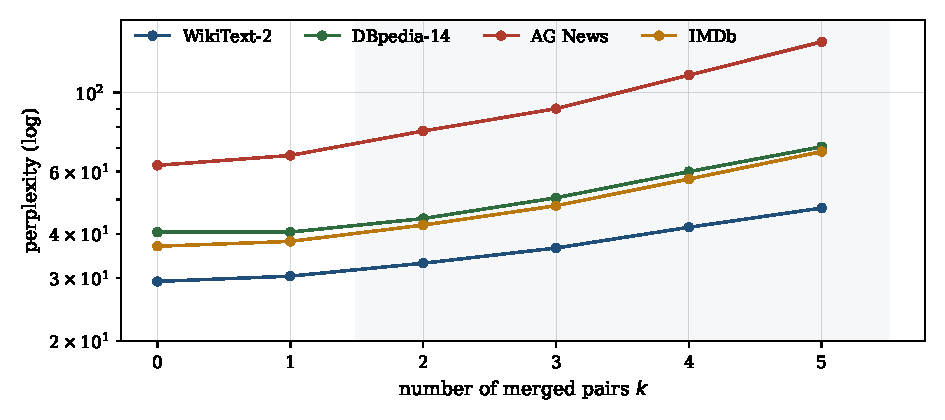
\includegraphics[width=0.98\textwidth]{figures/fig_expA_matrix.pdf}
\caption{Experiment~A: learned-model perplexity by number of merged pairs $k$,
per dataset (log scale). The curves rise smoothly with depth, and at $k{=}5$
the learned model stays far below the \dropfirst{} control on every dataset
($98.41$--$173.99$, Table~\ref{tab:unseen}).}
\label{fig:expA-matrix}
\end{figure}

\begin{figure}[t]
\centering
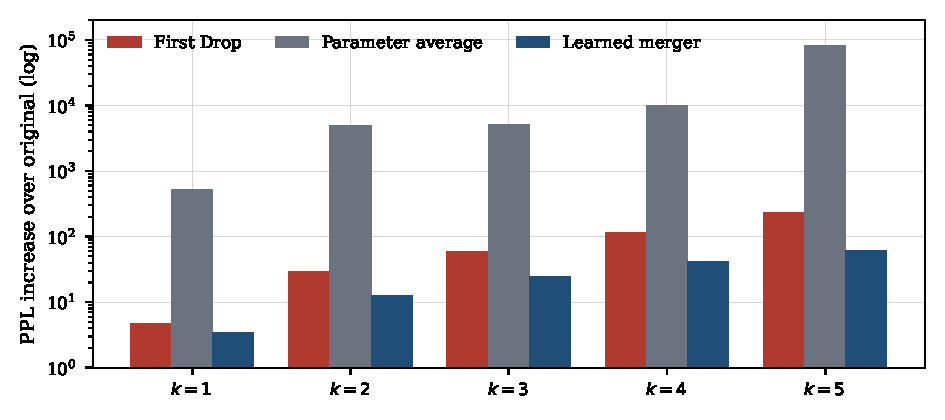
\includegraphics[width=0.98\textwidth]{figures/fig_expA_baseline.pdf}
\caption{Experiment~A: perplexity increase over the original GPT-2 on
WikiText-2 validation for the three methods at $k{=}1\dots5$ (log scale).
Parameter averaging collapses immediately; the learned merger stays below
\dropfirst{} at every level.}
\label{fig:expA-baseline}
\end{figure}

\paragraph{Preflight checks.} Asserted and recorded before training: (i)
\texttt{pack}/\texttt{unpack} round-trips for every kind; (ii)
\texttt{teacher\_states}$\circ\mathrm{LN}_f$ equals the model's own
\texttt{last\_hidden\_state}; (iii) every generated pair equals \dropfirst{}
exactly at initialisation ($\mathrm{rtol}=0$); (iv) a joint learned plan equals
the matching \dropfirst{} plan at initialisation; (v) the KL of identical models
is zero; and (vi) every generated second-block tensor receives a finite non-zero
gradient while all GPT-2 parameters receive none.

\paragraph{System effort and demonstration assets.} The system covers dataset
preparation, weight patching, differentiable weight generation, dual-GPU
optimisation, model reconstruction and evaluation. A live demo can load a saved
pair replacement, re-run the frozen-teacher checks, and compare the original
model, the drop baselines, parameter averaging and the learned weights on the
same tokens; the saved tables and plots show the one-to-five-merge trade-off
without any retraining during the demonstration.

%==============================================================================
\subsection{Experiment B: Multi-Step Operator Comparison}
\label{sec:expB}

\paragraph{Idea.} Treat compression as a sequence of five steps. At every step
we enumerate every boundary between currently adjacent groups, apply one of
four operators, and keep the candidate that minimises exact WikiText-2
validation NLL. The only thing that changes between runs is the operator
itself, which is what makes the comparison clean.

\paragraph{Operators.} A plan is a tuple of contiguous groups
$G=(g_1,\dots,g_m)$; a step merges $(g_b,g_{b+1})$ into $g_b\cup g_{b+1}$.
\begin{itemize}
  \item \removeop{}: group $[i,j]$ is replaced by its first block, $\hat B=B_i$.
  \item \averageop{}: every tensor is averaged over the group's \emph{original}
    blocks, $\hat\theta = \frac{1}{j-i+1}\sum_{\ell=i}^{j}\theta_\ell$.
  \item \linop{} (affine composition): for a span $[i,j]$ collect input/output
    activations $(X_\ell,Y_\ell)$ at each boundary and fit, per consecutive pair,
    a ridge-regularised affine map
    \begin{equation}
    A^\star,b^\star = \operatorname*{arg\,min}_{A,b}\;
    \lVert X_cA-Y_c\rVert_F^2 + \lambda\lVert A\rVert_F^2,\quad
    \lambda = \rho\,\frac{\operatorname{tr}(X_c^\top X_c)}{d},
    \end{equation}
    solved by Cholesky on $(X_c^\top X_c+\lambda I)A = X_c^\top Y_c$ and
    $b=\bar y-\bar xA$, with $\rho=10^{-4}$. Per-layer maps compose into one span
    map $A_{\text{tot}} \leftarrow A_{\text{tot}}A$,
    $b_{\text{tot}} \leftarrow b_{\text{tot}}A + b$, so the group becomes one
    affine block $\hat B(x)=A_{\text{tot}}x+b_{\text{tot}}$.
  \item \nlop{}: a new trainable GPT-2 block, initialised from the \emph{current}
    left merged block, so chains \texttt{1-2}$\to$\texttt{1-3} start from the
    already-learned block and learn the full original span; only its parameters
    receive gradients.
\end{itemize}

\paragraph{Objectives for the learnable block.} With teacher input $h$ and output
$h^\star$, the student block maps $h\mapsto\hat h$; the hidden loss is a
scale-normalised MSE (teacher-forced) and the distillation term at $T=2$ is
\begin{equation}
\mathcal{L}_{\text{hid}} = \frac{\lVert \hat h - h^\star\rVert_F^2 / N}
{\lVert h^\star\rVert_F^2 / N + \epsilon},\;\;
\mathcal{L}_{\text{KL}} = T^2 \cdot \frac{1}{N}\sum_{n}
\mathrm{KL}\!\left(p^t_n \,\lVert\, p^s_n\right),\;\;
\mathcal{L} = \lambda_{\text{hid}}\mathcal{L}_{\text{hid}}
+ \lambda_{\text{KL}}\mathcal{L}_{\text{KL}},
\end{equation}
with $\epsilon=10^{-8}$, $\lambda_{\text{hid}}=\lambda_{\text{KL}}=1$, and no
ground-truth CE. Optimisation: AdamW, LR $3\times10^{-5}$, weight decay $0.01$,
gradient clipping $1.0$, at most $15$ epochs with patience $15$; epoch $0$
evaluates the untrained block. Data budgets: $20{,}480$ local tokens
($\mathcal{L}_{\text{hid}}$), $20{,}480$ distillation tokens
($\mathcal{L}_{\text{KL}}$) and $4{,}096$ holdout tokens, all from the WikiText-2
\emph{train} split.

\begin{table}[t]
\centering
\small
\begin{tabular}{rrr}
\toprule
Epoch & Holdout total loss & New best \\
\midrule
$0$  & $0.2696$ & $0.2696$ \\
$3$  & $0.1549$ & $0.1549$ \\
$6$  & $0.1291$ & $0.1291$ \\
$9$  & $0.1238$ & $0.1238$ \\
$12$ & $0.1174$ & $0.1174$ \\
$15$ & $0.1136$ & $0.1136$ \\
\bottomrule
\end{tabular}
\caption{Experiment~B ablation over nonlinear training length for the selected
stage-$1$ span $0\text{-}1$ on the train-only holdout; epoch $15$ is selected.
This is the only hyperparameter ablated.}
\label{tab:ablation-b}
\end{table}

\paragraph{Results: in-domain selection.} Table~\ref{tab:hiro-val} reports the
chosen plan and WikiText-2 validation perplexity at each stage (original
$28.61$). At one step \nlop{} on blocks $0\text{-}1$ reaches $29.40$ and
\removeop{} reaches $30.01$, whereas \averageop{} and \linop{} already cost
$47.10$ and $36.36$. After five steps \removeop{} and \nlop{} are the only
methods below $100$ perplexity. Plans mix disjoint and chained merges.

\begin{table}[t]
\centering
\small
\begin{tabular}{clrr}
\toprule
Step & Method & Chosen plan & Val PPL \\
\midrule
$0$ & Original & -- & $28.61$ \\
\midrule
$1$ & \linop{}    & $6\text{-}7$ & $36.36$ \\
$1$ & \removeop{}            & $0\text{-}1$ & $30.01$ \\
$1$ & \averageop{}           & $7\text{-}8$ & $47.10$ \\
$1$ & \nlop{} & $0\text{-}1$ & $\mathbf{29.40}$ \\
\midrule
$2$ & \linop{}    & $6\text{-}8$ & $44.79$ \\
$2$ & \removeop{}            & $0\text{-}1;8\text{-}9$ & $35.12$ \\
$2$ & \averageop{}           & $6\text{-}8$ & $76.03$ \\
$2$ & \nlop{} & $0\text{-}1;3\text{-}4$ & -- \\
\midrule
$3$ & \linop{}    & $6\text{-}9$ & $60.75$ \\
$3$ & \removeop{}            & $0\text{-}1;2\text{-}3;8\text{-}9$ & $43.07$ \\
$3$ & \averageop{}           & $5\text{-}8$ & $138.96$ \\
$3$ & \nlop{} & $0\text{-}1;3\text{-}4;7\text{-}8$ & -- \\
\midrule
$4$ & \linop{}    & $1\text{-}2;6\text{-}9$ & $87.22$ \\
$4$ & \removeop{}            & $0\text{-}1;2\text{-}3;7\text{-}9$ & $58.03$ \\
$4$ & \averageop{}           & $4\text{-}8$ & $238.95$ \\
$4$ & \nlop{} & $0\text{-}1;3\text{-}4;5\text{-}6;7\text{-}8$ & -- \\
\midrule
$5$ & \linop{}    & $1\text{-}3;6\text{-}9$ & $122.05$ \\
$5$ & \removeop{}            & $0\text{-}1;2\text{-}3;5\text{-}6;7\text{-}9$ & $89.10$ \\
$5$ & \averageop{}           & $3\text{-}8$ & $424.98$ \\
$5$ & \nlop{} & $0\text{-}1;3\text{-}4;5\text{-}6;7\text{-}8;9\text{-}10$ & -- \\
\bottomrule
\end{tabular}
\caption{Experiment~B chosen plan and WikiText-2 validation PPL by step. The
\nlop{} stage-$1$ score is $29.4023$; its stage-$2$--$5$ validation numbers were
not captured (marked \texttt{--}); their quality is reported on unseen data.}
\label{tab:hiro-val}
\end{table}

\paragraph{Results: complete unseen-test matrix.} Table~\ref{tab:matrices}
gives the $5\text{-stage}\times4\text{-method}$ unseen
perplexity matrix per dataset. \nlop{} is the best method at every stage on AG
News and IMDb, and from stage $2$ onward on DBpedia; the single exception is
DBpedia stage $1$, where \removeop{} edges it by $0.03$.

\begin{table}[t]
\centering
\small
\begin{minipage}[t]{0.48\textwidth}
\centering
\begin{tabular}{lrrrr}
\toprule
\multicolumn{5}{c}{\textbf{DBpedia-14} (orig.\ $30.99$)}\\
\cmidrule(lr){1-5}
Stage & Remove & Avg. & Linear & Nonlin. \\
\midrule
$1$ & $\mathbf{32.24}$ & $52.65$ & $52.29$ & $32.27$ \\
$2$ & $36.99$ & $88.29$ & $67.42$ & $\mathbf{35.53}$ \\
$3$ & $43.83$ & $153.47$& $108.49$& $\mathbf{40.78}$ \\
$4$ & $57.64$ & $246.82$& $191.19$& $\mathbf{50.07}$ \\
$5$ & $85.17$ & $424.94$& $294.50$& $\mathbf{59.81}$ \\
\bottomrule
\end{tabular}
\end{minipage}\hfill
\begin{minipage}[t]{0.48\textwidth}
\centering
\begin{tabular}{lrrrr}
\toprule
\multicolumn{5}{c}{\textbf{AG News} (orig.\ $51.82$)}\\
\cmidrule(lr){1-5}
Stage & Remove & Avg. & Linear & Nonlin. \\
\midrule
$1$ & $53.34$ & $88.67$ & $96.83$ & $\mathbf{53.04}$ \\
$2$ & $62.78$ & $146.54$& $131.50$& $\mathbf{63.19}$ \\
$3$ & $78.18$ & $249.51$& $211.44$& $\mathbf{72.98}$ \\
$4$ & $104.43$& $381.09$& $394.92$& $\mathbf{96.04}$ \\
$5$ & $150.97$& $569.19$& $613.16$& $\mathbf{115.97}$\\
\bottomrule
\end{tabular}
\end{minipage}

\vspace{0.6em}
\begin{minipage}[t]{0.48\textwidth}
\centering
\begin{tabular}{lrrrr}
\toprule
\multicolumn{5}{c}{\textbf{IMDb} (orig.\ $37.20$)}\\
\cmidrule(lr){1-5}
Stage & Remove & Avg. & Linear & Nonlin. \\
\midrule
$1$ & $38.47$ & $55.02$ & $53.00$ & $\mathbf{38.31}$ \\
$2$ & $42.76$ & $84.65$ & $70.58$ & $\mathbf{41.97}$ \\
$3$ & $52.20$ & $133.21$& $105.11$& $\mathbf{46.84}$ \\
$4$ & $65.77$ & $201.24$& $183.09$& $\mathbf{55.63}$ \\
$5$ & $85.12$ & $310.88$& $282.00$& $\mathbf{66.03}$ \\
\bottomrule
\end{tabular}
\end{minipage}\hfill
\begin{minipage}[t]{0.48\textwidth}
\centering
\begin{tabular}{llrrrr}
\toprule
\multicolumn{6}{c}{\textbf{Relative degradation (\%)}}\\
\cmidrule(lr){1-6}
Data & St. & Rem. & Avg. & Lin. & Non. \\
\midrule
DBp. & $1$ & $\mathbf{4.0}$ & $69.9$ & $68.7$ & $4.1$ \\
DBp. & $5$ & $174.8$ & $1271.1$ & $850.2$ & $\mathbf{93.0}$ \\
AG & $1$ & $2.9$ & $71.1$ & $86.9$ & $\mathbf{2.4}$ \\
AG & $5$ & $191.4$ & $998.5$ & $1083.3$ & $\mathbf{123.8}$ \\
IMDb & $1$ & $3.4$ & $47.9$ & $42.5$ & $\mathbf{3.0}$ \\
IMDb & $5$ & $128.8$ & $735.6$ & $658.0$ & $\mathbf{77.5}$ \\
\bottomrule
\end{tabular}
\end{minipage}
\caption{Experiment~B unseen perplexity by dataset (top) and relative
degradation versus each corpus's original (bottom). Best per row in bold.}
\label{tab:matrices}
\end{table}

\paragraph{Structural verification.} Five self-checks run on a randomly
initialised tiny GPT-2 before any compression: (i) disjoint and chained plans
are reconstructed consistently; (ii) multi-step removal keeps exactly the
intended first block; (iii) averaging is uniform over original blocks; (iv) a
nonlinear block is initialised from the current left merged block; and (v) only
the newly created block has \texttt{requires\_grad}. Config, plans and
checkpoints are hash-locked and the unseen test is run exactly once.

%==============================================================================
\subsection{Experiment C: Affine Merging with SG-SC and CGOS}
\label{sec:expC}

\paragraph{Idea.} Treat each block as an affine map, then ask three questions
about it. Do the obvious fixed operators (deletion, averaging, plain
composition) hold up? Does replacing the fixed rule with a similarity-gated,
error-weighted SLERP version (SG-SC) help? And can a calibration-based selector
(CGOS) pick the right operator per pair without extra hyperparameters?

\paragraph{Affine composition.} Using a row-vector convention a block is
$M_\ell(x)=x A_\ell + b_\ell$. For adjacent maps $(A_1,b_1)$ and $(A_2,b_2)$:
\begin{equation}
\removeop: (A,b)=(A_2,b_2),\quad
\averageop: (A,b)=\left(\tfrac{A_1+A_2}{2},\,\tfrac{b_1+b_2}{2}\right),\quad
\text{Multiply}: (A,b)=(A_1A_2,\; b_1A_2 + b_2).
\end{equation}
Random-Weight Average (RWA) permutes the entries of the second map within each
tensor while preserving its distribution before the $50$--$50$ average.

\paragraph{SG-SC.} Similarity-Gated, Error-Weighted SLERP Composition combines a
compatibility gate (equally weighted CKA and cosine similarity of pooled
hidden-state means) with calibration errors from \averageop{} and Multiply to set
the interpolation weight, after which
\begin{equation}
\slerp(a,b;w)=\frac{\sin((1-w)\theta)}{\sin\theta}a+\frac{\sin(w\theta)}{\sin\theta}b,
\qquad \theta=\arccos\!\frac{a\cdot b}{\lVert a\rVert\lVert b\rVert}.
\end{equation}

\paragraph{CGOS.} Calibration-Guided Operator Selection computes, per adjacent
pair, the calibration hidden-state reconstruction error of \removeop{},
\averageop{} and Multiply, and selects the smallest-error operator; it adds no
hyperparameters, CKA, SLERP or interpolation.

\paragraph{Protocol and results.} Affine maps are fitted on a training portion;
diagnostics for CGOS come from a separate calibration portion; validation
perplexity ranks the candidates; one joint selection then fixes the final
configuration, and the test set is used once, at the very end. The FULL
configuration uses $20{,}000$ fit tokens, $20{,}000$ calibration tokens and
$50{,}000$ eval tokens; RWA averages five random runs; latency is measured over
$30$ repetitions at seed $42$ in float32. The joint selection picks
\textbf{Multiply for pair $6$--$7$}, at validation $\mathrm{PPL}=41.5146$ and
test $\mathrm{PPL}=47.9306$ (original test $38.4868$), with $10.917\%$ parameter
reduction and compressed latency $18.51\pm0.41$\,ms versus $22.73\pm5.07$\,ms
baseline; CGOS agrees with the validation-best operator on $9$ of $11$ pairs
($81.82\%$).

\begin{table}[t]
\centering
\small
\begin{tabular}{llrl}
\toprule
Metric & Value & Metric & Value \\
\midrule
Original test PPL & $38.4868$ & Compressed parameters & $110{,}854{,}656$ \\
Selected pair & $6$--$7$ & Parameter reduction & $10.917\%$ \\
Selected method & Multiply & Compressed latency & $18.51\pm0.41$\,ms \\
Selected validation PPL & $41.5146$ & Baseline latency & $22.73\pm5.07$\,ms \\
Final test PPL & $47.9306$ & CGOS agreement & $9/11 = 81.82\%$ \\
\bottomrule
\end{tabular}
\caption{Experiment~C FULL-run summary (GPT-2, WikiText-2, all $11$ pairs).}
\label{tab:lingala}
\end{table}

%==============================================================================
\subsection{Experiment D: Calibrated Similarity-Guided SLERP}
\label{sec:expD}

\paragraph{Idea.} The idea is to let the model tell us which pair to merge,
rather than guessing. Adjacent pairs are ranked by how similar their hidden
states are, the chosen pair is merged with SLERP at a weight tuned on a handful
of calibration tokens---separate weights for attention and MLP---and the
process repeats, with no gradient training anywhere.

\paragraph{Method.} For every adjacent pair $(L,L{+}1)$ we compute linear CKA
and the cosine similarity of their z-scored block outputs and fold them into a
single score $S$; the top-$k$ pairs are shortlisted. The merge initialises the
SLERP weight from a similarity prior $w=g(S)$, then tunes it on the calibration
set with per-group weights $w_\text{attn}, w_\text{mlp}$ and a mode search over
\{SLERP, LERP\}. Calibration draws ${\sim}4$k tokens for similarity and
${\sim}8$k tokens for tuning, all from the WikiText-2 \emph{train} split. The
procedure is greedy and iterative: after each merge the similarities are
recomputed on the new model.

\paragraph{Results.} Table~\ref{tab:sravan} summarises the runs. On the
calibration-selected pair the fixed-$0.5$ linear merge collapses
($\mathrm{val}\ 111.36$) and affine Multiply lands at $53.32$; the calibrated
SLERP (OURS) reaches $\mathrm{val}=38.30$ and $\mathrm{test}=43.85$ at one
merge---within a point of deletion's own $\mathrm{val}=40.87$, but with a smooth
interpolant in between instead of a hard spatial cut. Pushing to four merges
degrades the val to $59.17$ (test $66.88$), a gentler slope than either the
linear or the affine route.

\begin{table}[t]
\centering
\small
\begin{tabular}{lrrrr}
\toprule
Method & Merges & Params & Val PPL & Test PPL \\
\midrule
Original GPT-2 & $0$ & $124{,}439{,}808$ & $33.94$ & $38.83$ \\
A1: remove layer 5 & $1$ & $117{,}351{,}936$ & $40.87$ & $46.69$ \\
A1: linear average $0.5$ & $1$ & $117{,}351{,}936$ & $111.36$ & $120.59$ \\
A1: affine multiply & $1$ & $110{,}854{,}656$ & $53.32$ & $57.47$ \\
OURS (calibrated SLERP) & $1$ & $117{,}351{,}936$ & $\mathbf{38.30}$ & $\mathbf{43.85}$ \\
OURS & $2$ & $110{,}264{,}064$ & $41.80$ & $47.25$ \\
OURS & $3$ & $103{,}176{,}192$ & $48.66$ & $55.27$ \\
OURS & $4$ & $96{,}088{,}320$ & $59.17$ & $66.88$ \\
\bottomrule
\end{tabular}
\caption{Experiment~D summary. The selected pair is $3$--$4$ with similarity
$S=0.951$ and a tuned weight $w=1.0$.}
\label{tab:sravan}
\end{table}

%==============================================================================
\subsection{Foundational Exploration: Design-Space Map, Results and Limits}
\label{sec:foundation}

The first author ran a broad, \emph{tangential} exploration that enumerated and
stressed the projects and techniques on which the four primary experiments are
built, producing the reference baselines and the reproducibility methodology
shared by the whole group. Fifteen approaches spanning eight mechanism
families (influence-based removal, low-rank/bridge replacement, quantization,
weight merging, parameter tying, distillation, learned sparsity/structured
pruning, and adaptive depth) were implemented and probed on two architecturally
unlike models, GPT-2 small and SmolLM-135M. Four produced usable results
---the fitted ternary bridge, the Block-Influence control, SVD low-rank and the
quantized no-op bypass; distillation repair and LayerDrop produced results only
after a budgeted re-run with per-fit seeds; the affine-bridge,
permutation-averaging, weight-merging and weight-tying variants failed at
increasing multiples of perplexity; and the remaining notebooks stayed scaffolds
at the exploration's compute budget. The per-approach artefacts, negative
results and the full results table are archived under
\url{https://github.com/sumitjhaa/gpt2-layermerging/tree/main/Assignment2};
we quote only the numbers that survived our own audit below.

\begin{figure}[t]
\centering
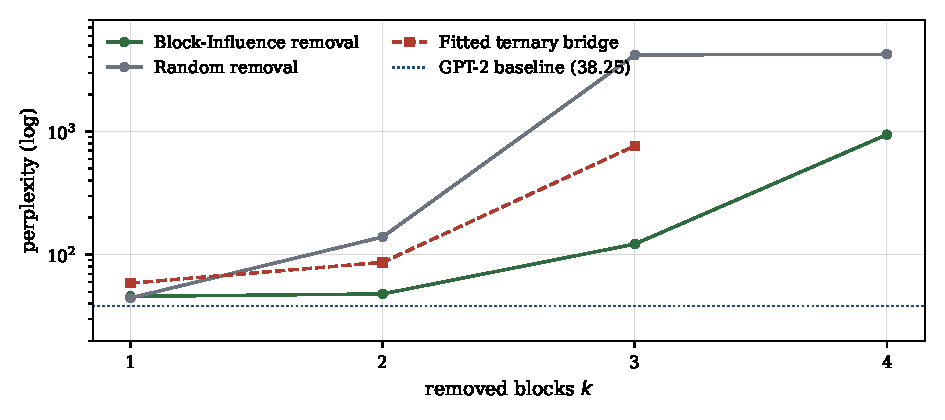
\includegraphics[width=0.98\textwidth]{figures/fig_foundation.pdf}
\caption{Foundational exploration on GPT-2: perplexity of Block-Influence
removal, random removal and the fitted ternary bridge at $k{=}1\dots4$ against
the $38.25$ baseline (log scale). BI removal is the only rule that survives
beyond $k{=}2$; the bridge loses to deletion at identical parameter counts.}
\label{fig:foundation}
\end{figure}

\paragraph{Block Influence and controlled removal.} For every decoder block
$\mathrm{BI}_l = 1-\cos(h_\text{in}^{(l)},h_\text{out}^{(l)})$, computed from one
forward pass; low BI means near-identity. The rankings are GPT-2: $4,1,2,3,5$ and
SmolLM-135M: $2,27,5,4,3$ (most to least redundant). Targeted removal beats
\emph{random} removal decisively for $k\ge2$ (see Figure~\ref{fig:foundation}) (GPT-2 $k{=}2$: $47.95$ vs.\
$139.09$; $k{=}3$: $121.81$ vs.\ $4181.21$; $k{=}4$: $943.24$ vs.\ $4237.94$;
SmolLM $k{=}3$: $29.91$ vs.\ $34.23$; $k{=}4$: $34.20$ vs.\ $57.37$), while
$k{=}1$ is cheap either way. This is the controlled evidence that BI ranking is
what makes pruning cheap, and it is the null control used throughout.

\paragraph{Fitted ternary bridge (\term{}).} Replacing a redundant block by a
bridge $f(x)=x+xUV$ with $U,V$ \emph{fitted} on captured $(X,Y)$ pairs,
$\min_{U,V}\lVert XUV-(Y-X)\rVert_F^2$ (Adam, $80$ iters), then AbsMean-quantised
to $\{-1,0,+1\}\gamma$ \citep{ma2024bitnet}, is the headline exploration result.
It produces \emph{identical} parameter counts to plain deletion (a rank-$32$
bridge is $49{,}152$ weights standing in for a $7.1$M block) and keeps the graph
depth while shrinking the replaced weights to ${\sim}1.58$ bit/param. Under
per-fit seeding it is clearly worse than deletion (GPT-2 $k{=}1$:
$58.67\pm9.53$ vs.\ $45.76$; SmolLM $30.77\pm3.54$ vs.\ $19.93$). Its value is
representational rather than a perplexity win: the computation graph keeps its
full depth while the replaced weights shrink to ${\sim}1.58$ bit/param.
Single-seed sweeps over rank, bits and
calibration text confirm the picture and add one nuance
(Table~\ref{tab:foundation-abl}): giving the bridge more capacity makes GPT-2
perplexity \emph{worse}, and enlarging the fit text from $2$k to $20$k
characters is the only axis that clearly helps---GPT-2 drops to $47.86$, still
above deletion's $45.76$.

\paragraph{Repair and LayerDrop.} Pruned distillation
$\mathcal{L}=\alpha\,\ce + (1-\alpha)T^2\mathrm{KL}$ \citep{ma2023llmpruner}
recovers a large fraction of the deletion cost at no parameter cost (healed beat
pruned in $12/12$ runs), and LayerDrop \citep{fan2020layerdrop} is the strongest
method on SmolLM-135M and the only configuration that lands \emph{below} its own
unpruned baseline ($15.54\pm0.01$ vs.\ $16.39$)---evidence that the best method
is \emph{model-dependent} (Table~\ref{tab:foundation-repair}).

\paragraph{Supporting rules.} An SVD low-rank surrogate on SmolLM equals the
baseline at rank $256$ ($19.93$), gives $22.00$ at $128$ and $24.22$ at $64$. The
quantized no-op bypass shows the three lowest-BI layers survive $2$-bit
quantization with no perplexity change (SmolLM L5: $17.76\!\to\!17.76$), so the
same ranking predicts both removability and quantization tolerance. A
training-free SVD diagnostic forms the residual map $\Delta=Y-X$ and shows Block
Influence and residual low-rankness are \emph{different} properties (lowest-BI
GPT-2 block L4 has rank-$32$ explained variance $0.392$ while L1 has $0.875$),
explaining why local affine fitting improves while end-task perplexity can
degrade.

\begin{table}[t]
\centering
\small
\begin{tabular}{llrrrr}
\toprule
Model & Operator & $k{=}1$ & $k{=}2$ & $k{=}3$ & $k{=}4$ \\
\midrule
GPT-2 & baseline & \multicolumn{4}{c}{$38.25$} \\
GPT-2 & BI removal & $45.76$ & $47.95$ & $121.81$ & $943.24$ \\
GPT-2 & random removal & $44.42$ & $139.09$ & $4181.21$ & $4237.94$ \\
GPT-2 & fitted ternary bridge & $58.67$ & $86.49$ & $765.21$ & --- \\
\midrule
SmolLM & baseline & \multicolumn{4}{c}{$16.39$} \\
SmolLM & BI removal & $19.93$ & $26.13$ & $29.91$ & $34.20$ \\
SmolLM & random removal & $20.83$ & $26.37$ & $34.23$ & $57.37$ \\
SmolLM & fitted ternary bridge & $30.77$ & $41.77$ & $58.21$ & --- \\
\bottomrule
\end{tabular}
\caption{Foundational exploration: the fitted ternary bridge loses to deletion
at identical parameter counts, while the BI ranking beats random removal from
$k\ge2$ (all GPT-2 bridge/random values are 3-seed; the earlier single-seed
$\term{}$ value $45.11$ came from an unreproducible global-RNG run and is
superseded).}
\label{tab:foundation}
\end{table}

\begin{table}[t]
\centering
\small
\begin{tabular}{llrrr}
\toprule
Model & Method & $k{=}1$ & $k{=}2$ & Recovered \\
\midrule
GPT-2 & BI removal (pruned) & $45.76$ & $47.95$ & --- \\
GPT-2 & BI $+$ distillation & $\mathbf{41.68}$ & $\mathbf{44.06}$ & $54.3\%$ \\
GPT-2 & LayerDrop & $51.74$ & $57.53$ & --- \\
\midrule
SmolLM & BI removal (pruned) & $19.93$ & $26.13$ & --- \\
SmolLM & BI $+$ distillation & $18.67$ & $22.14$ & $34.9\%$ \\
SmolLM & LayerDrop & $\mathbf{15.54}$ & $\mathbf{19.62}$ & beats baseline \\
\bottomrule
\end{tabular}
\caption{Foundational exploration: repair and LayerDrop (validation perplexity,
mean over three seeds). LayerDrop alone beats its own $16.39$ baseline on SmolLM;
distillation wins on GPT-2.}
\label{tab:foundation-repair}
\end{table}

\begin{table}[t]
\centering
\small
\begin{tabular}{llrr}
\toprule
Sweep & Value & GPT-2 PPL & SmolLM PPL \\
\midrule
Bridge rank & $4 $ & $50.57$ & $26.54$ \\
            & $16$ & $60.35$ & $25.22$ \\
            & $64$ & $68.18$ & $26.02$ \\
            & $128$ & $341.10$ & $32.83$ \\
\midrule
Quant.\ bits & $2$ & $52.35$ & $34.83$ \\
            & $4$ & $69.78$ & $44.02$ \\
            & $8$ & $69.72$ & $39.55$ \\
\midrule
Calib.\ text & $2$k chars & $67.45$ & $32.92$ \\
            & $20$k chars & $47.86$ & $24.12$ \\
\bottomrule
\end{tabular}
\caption{Foundational exploration, single-seed sweeps on the fitted bridge at
$k{=}1$: bridge rank, AbsMean quantisation bits, and calibration text length
(one axis changes at a time). Deletion sits at $45.76$ (GPT-2) and $19.93$
(SmolLM). More bridge capacity makes GPT-2 perplexity \emph{worse}, while the
larger calibration text is the only axis that clearly helps.}
\label{tab:foundation-abl}
\end{table}

\paragraph{Reproducibility audit.} A global-RNG defect was found and fixed: the
same configuration gave $47.67/27.04$ when re-executed alone but $47.95/27.67$
when reached by running the notebook top to bottom. Every stochastic fit is now
driven from an explicit per-fit \texttt{torch.Generator}, and a closing audit of
thirteen structural invariants refuses to certify output unless all hold.

\paragraph{Limitations of the foundational exploration.}
\emph{(i) Compute.} All fifteen approaches ran on a single free Apple-Silicon
MPS laptop with no paid GPU and training budgets capped at $60$--$80$ steps;
consequently several training-heavy approaches (KD repair, KD student, learned
$L_0$ gates, LayerDrop as first implemented, early exit) produced no separable
results and are reported as archived scaffolds rather than findings.
\emph{(ii) Confounded bridge.} The bridge is rank-$32$ \emph{and} $2$-bit
simultaneously and no unquantized float32 control was run, so the honest
claim is narrow (``this particular linear-plus-residual form loses to deletion,
and giving it more capacity did not help''), not ``low-rank replacement loses''.
\emph{(iii) Broken GPT-2 SVD row.} The GPT-2 SVD row is flat at $36.78$ because a
dtype guard swallowed the weight edit; it needs an explicit \texttt{.float()}
rerun and is unusable as evidence. \emph{(iv) Noisy quantization trend.} The
GPT-2 quantization trend is invisible at the $3$k-token evaluation budget and is
eval noise. \emph{(v) Protocol mismatch.} The exploration uses $256$-token
non-overlapping windows over a $3$k-token budget, whereas A--D use exact
sliding-window evaluation, so these numbers are \emph{not} directly comparable to
A--D and are used qualitatively. \emph{(vi) Single-seed ablations.} The rank and
bitwidth sweeps are single-seed and should be read as indicative. \emph{(vii)
Superseded numbers.} The early single-seed bridge value ($45.11$ at $k{=}1$) came
from the global-RNG configuration and was replaced by the per-fit-seeded runs.
These limits are the reason the exploration is presented as the \emph{map} of the
design space rather than as a competing headline method.

%==============================================================================
\subsection{Additional Pilot: Closed-Form Training-Free Merges}
\label{sec:pilot}

A closed-form, training-free pilot explored three further mechanisms on GPT-2
(quick-mode: $8192$ fit tokens, one seed; the full $50$k-token/three-seed grid is
pending). \emph{Remove-and-Patch (R\&P)} keeps one real block and replaces the
other by a mean plus a fitted low-rank correction $y=x+\mu+(x-\bar x)D_r$ with
$D_r$ from the top-$r$ right singular vectors of $X_cD_\text{ols}$
(Eckart--Young), stored factored as $(U,V)$. \emph{Union-Select-Reconstruct
(USR)} scores all $6144$ MLP neurons of both blocks by
$s=\mathbb{E}[a^2]\lVert o\rVert^2$, keeps the top $3072$, and re-solves the
readout with shrinkage. \emph{Correlation-Guided Neuron Fusion} pairs neurons by
Pearson correlation, averages their inputs and jointly refits outputs. In the
quick run R\&P reaches the best per-pair validation values (e.g.\ pair
$2$--$3$: $32.44$), random-subspace and random-pairing controls are uniformly
worse (validating the learned structure), and pair-local normalised MSE predicts
end-to-end damage (Spearman $0.814$); early-pair ($0$--$1$) merges are
catastrophic for every method. These numbers are preliminary.

%==============================================================================
\subsection{Cross-Experiment Analysis and Merged Results}
\label{sec:merged}

Because the four experiments used different but related exact evaluators
(different window sizes, strides and token caps), absolute perplexities are not
directly comparable across experiments; we therefore compare methods
\emph{within} each experiment and only look at orderings that repeat. Three
patterns came up over and over across the portfolio.

\paragraph{(1) Learned fusion dominates at depth.} In Experiment~B \nlop{} is
best in $14$ of $15$ unseen stage$\times$dataset cells; in Experiment~A the
guarded learned merger beats \dropfirst{} at every $k$ on the ranking holdout
(CE gap $-0.025$ to $-0.805$ nats) and on IMDb by $68.23$ vs.\ $90.52$ at
$k{=}5$. Training-free operators fall behind increasingly with depth.

\paragraph{(2) Averaging is unusable.} \averageop{} reaches $+1271.1\%$ on
DBpedia at stage $5$ (B), $\mathrm{val}=111.36$ at a single merge (D), and
$10^2$--$10^3\times$ baseline in the foundational sweep. The mechanism is the
neuron-permutation mismatch between adjacent blocks, which the learned/calibrated
operators explicitly repair.

\paragraph{(3) The best training-free rule is model- and pair-dependent.} Affine
Multiply is best on pair $6$--$7$ under CGOS (C); calibrated SLERP is best at one
merge under similarity selection (D); in the foundational study LayerDrop wins on
SmolLM while distillation wins on GPT-2. No single universal rule is supported.

\begin{table}[t]
\centering
\footnotesize
\begin{tabular}{L{1.0cm} L{2.7cm} L{2.7cm} L{2.5cm} L{4.5cm}}
\toprule
Exp. & Family & Best artifact & Selection signal & Key result \\
\midrule
A & Learnable, weight-space & Hypernetwork correction & Guarded ranking
  & IMDb $68.23$ vs.\ $90.52$ at $k{=}5$ ($28.48\%$ removed) \\
B & Learnable, activation-space & Nonlinear block & Exact validation NLL
  & Best in $14/15$ unseen cells; IMDb $+77.5\%$ vs.\ deletion $+128.8\%$ \\
C & Affine $+$ selection & Multiply on $6$--$7$ (CGOS) & Calib.\ recon.\ error
  & Test $47.93$ at $10.92\%$ reduction; CGOS agrees $9/11$ \\
D & Interpolation & Calibrated SLERP & Similarity $+$ calibration
  & Val $38.30$ / test $43.85$ at one merge \\
Found. & Reference baselines & BI removal $+$ distillation & Validation NLL
  & Recovers $54.3\%$ of deletion cost on GPT-2 \\
Pilot & Closed-form & Remove-and-Patch & Validation PPL
  & Best per-pair values; controls worse (quick run) \\
\bottomrule
\end{tabular}
\caption{Headline configuration of each study on GPT-2. Absolute numbers are each
experiment's own protocol and are not mutually comparable; the ordering of
methods within an experiment is the reliable signal.}
\label{tab:merged}
\end{table}

%==============================================================================
\subsection{Discussion and Limitations}
\label{sec:limits}

\paragraph{Threats to validity.} First, the experiments use different exact
evaluators, so absolute perplexities are not mutually comparable and only
within-experiment orderings are claimed. Second, Experiment~A adapts a merger to
one GPT-2 checkpoint; its accuracy is next-\emph{token} BPE accuracy, not
whole-word; its ten passes mix single and joint tasks; and its additive-cost
selection is a surrogate that can miss a better joint plan. Third, Experiment~B's
selection is greedy and stage-wise and its \nlop{} stage-$2$--$5$ validation
numbers were not captured, so those in-domain curves are incomplete rather than
favourable. Fourth, Experiment~C evaluates one merge depth and one selected pair
and does not sweep the affine ridge; Experiment~D has no unseen-domain
evaluation in the reported runs and its results come from notebook artefacts.
Fifth, the pilot's numbers are quick-mode and single-seed, and the foundational
exploration's limits are itemised in Section~\ref{sec:foundation}. Sixth, the
guard in A and the hash lock in B are held-out \emph{selection} rules, not
guarantees on unseen domains. Seventh, we did not re-run FuseGPT, which has no
official release, so that comparison is qualitative. Finally, all experiments
share one backbone: no transfer to other checkpoints is claimed.

\paragraph{Cost.} Learnable methods (A, B) strictly cost more than training-free
ones; their advantage is a quality result, not a compute result. A's
$39.4$M-parameter merger is discarded at deployment. \linop{} (B) is the most
expensive training-free operator because it needs activation collection and a
Cholesky solve per span per stage.

\paragraph{Multilingual extension.} The mentor suggested applying the same
merges to multilingual models. Every operator here is backbone-agnostic, and a
multilingual checkpoint would test whether the fusion advantage survives richer
token statistics and faster LayerNorm/attention drift. We leave this to future
work.

\paragraph{Takeaways.} Putting the four experiments together, the story is
consistent. Once compression goes past one or two merges, something trained is
doing the work: the learnable methods (A, B) are the only ones that hold up at
depth, and their lead over training-free operators grows as more blocks are
removed. Averaging two blocks is not a merging strategy---the neurons simply do
not line up---except when an entire contiguous tail span is averaged, and even
then it is still beaten. Among training-free rules the winner depends on the
model and the pair: affine composition on one pair (C), calibrated SLERP on
another (D), LayerDrop on small models. That is why we report every per-pair
ranking rather than a single recipe. If we had to pick one cheap baseline to
reuse, it would be Block-Influence removal patched with distillation.

%==============================================================================
\subsection{Code and Reproducibility}
\label{sec:code}

Every method in this report was implemented from scratch by the group; no
external compression library was used. The tangential exploration and its full
results table (fifteen approaches, per-fit seeds, CSV dumps), the four
experiments, the pilot and the source of this document are all compiled in one
place:
\url{https://github.com/sumitjhaa/gpt2-layermerging/tree/main/Assignment2}.
Each experiment ships as a notebook with saved CSV artefacts, so every number
in Table~\ref{tab:merged} traces back to a raw run file rather than a
re-derivation.

\begin{itemize}
  \item \textbf{Tooling.} Standard Python/PyTorch with HuggingFace
    \texttt{transformers} and \texttt{datasets}; the dependency list sits beside
    each notebook. Pretrained weights (\texttt{openai-community/gpt2},
    \texttt{HuggingFaceTB/SmolLM-135M}) and WikiText-2 are downloaded and cached
    once.
  \item \textbf{Compute.} Experiment~A ran on two NVIDIA T4 GPUs with one frozen
    teacher and one merger replica per GPU; the other experiments and the
    exploration ran on a single GPU or an Apple-Silicon laptop under the budgets
    stated in their sections.
  \item \textbf{Determinism.} Every stochastic fit in the exploration is driven
    by an explicit per-fit \texttt{torch.Generator} seed since the global-RNG
    audit (Section~\ref{sec:foundation}); Experiment~B locks its protocol with
    SHA-256 hashes; Experiment~A asserts its six preflight checks before any
    training starts.
  \item \textbf{Data handling.} The DBpedia-14, AG News and IMDb shards are
    opened exactly once for final reporting, with the scored token positions
    recorded, so the unseen numbers can be re-checked without re-selecting.
\end{itemize}

%==============================================================================
\section{Team Contributions}
\label{sec:contrib}

The six members worked as one team on adjacent-layer merging. Following the
assignment's instruction to assign contributions fairly, and in recognition that
each member owned one mechanistically distinct experiment \emph{and} shared the
common protocol, we record an \textbf{equal contribution} for all six members
($100\%/6 \approx 16.67\%$ each). Table~\ref{tab:contrib} lists the members with
their roll numbers and primary deliverables; the paragraphs below give the
auditable detail.

\begin{table}[h]
\centering
\footnotesize
\begin{tabular}{L{3.6cm} L{1.7cm} L{7.4cm} L{1.2cm}}
\toprule
Member & Roll No. & Primary deliverable in this report & Share \\
\midrule
Sumit Kumar Jha & 26210180
  & Tangential exploration and reference baselines & \multirow{6}{*}{16.67\%} \\
Amrita Lodh & 26290001
  & Exp.~A: learnable weight-space merging & \\
Hiroyoshi Tsujimoto & 26210172
  & Exp.~B: four-operator iterative comparison & \\
Sura Sravan Kumar & 24110362
  & Exp.~D: calibrated SLERP merging & \\
Satvik Sharma & 26120008
  & Pilot: closed-form training-free merges & \\
Lingala Hasini & 24110186
  & Exp.~C: affine merging, SG-SC and CGOS & \\
\bottomrule
\end{tabular}
\caption{Team contribution summary. All six members contributed equally
($100\%/6 \approx 16.67\%$ each); the table lists each member's roll number and
primary deliverable in this unified report.}
\label{tab:contrib}
\end{table}

\begin{itemize}
  \item \textbf{Sumit Kumar Jha (equal, $16.67\%$).} Tangential exploration and
    design-space mapping: the fifteen-approach survey across eight families on
    GPT-2 and SmolLM-135M, the reference baselines (Block-Influence removal,
    distillation repair, LayerDrop), the fitted ternary bridge, the
    reproducibility and seed audit, the shared repository and evaluation
    protocol, and the integration and \LaTeX{} production of this merged
    report.
  \item \textbf{Amrita Lodh (equal, $16.67\%$).} Experiment~A: the
    second-block-anchored learnable weight-space merger (novelty, architecture
    and weight tokenisation, training objective, two-GPU synchronous schedule
    and batch auto-tuner, pair ranking and guarded selection), all
    Experiment~A experiments and analysis, and the Experiment~A report.
  \item \textbf{Hiroyoshi Tsujimoto (equal, $16.67\%$).} Experiment~B: the
    four-operator suite (removal, averaging, closed-form affine linear
    composition, and a trainable block), the exact sliding-window evaluator,
    the structural self-checks and hash-locked protocol, greedy stage-wise
    selection, the full three-dataset, five-stage, four-method unseen matrix,
    and the Experiment~B report.
  \item \textbf{Sura Sravan Kumar (equal, $16.67\%$).} Experiment~D: the
    calibrated, similarity-guided SLERP merger (CKA+cosine pair scoring,
    similarity-prior and calibrated per-group attention/MLP weights, mode
    search, greedy iteration), the comparison against MKA/CoM-style baselines,
    and the Experiment~D report.
  \item \textbf{Satvik Sharma (equal, $16.67\%$).} The closed-form
    training-free pilot: Union-Select-Reconstruct (USR), Remove-and-Patch
    (R\&P) and Correlation-Guided Neuron Fusion, with random-subspace and
    random-pairing controls, the pair-local nMSE predictor of end-to-end
    damage, and the pilot report.
  \item \textbf{Lingala Hasini (equal, $16.67\%$).} Experiment~C: affine
    merging, the Random-Weight-Average control, SG-SC and its ablations, CGOS
    calibration-guided operator selection, the FULL-run evaluation with
    latency measurement, and the Experiment~C report.
\end{itemize}

\paragraph{Shared.} Dataset protocol (WikiText-2 for training/selection;
DBpedia-14, AG News and IMDb for one-shot unseen testing), the common
baseline/SOTA framing, weekly mentor meetings, and cross-checking of each
other's numbers against the raw artefacts. Because the work of every member is
included in this single report, the group submits one unified document and all
members receive the same credit.

%==============================================================================
\bibliographystyle{acl_natbib}
\bibliography{references}

\end{document}
